\documentclass[border=10pt]{standalone}

\usepackage{tikz}
\usetikzlibrary{automata, positioning, fit, backgrounds}

\begin{document}

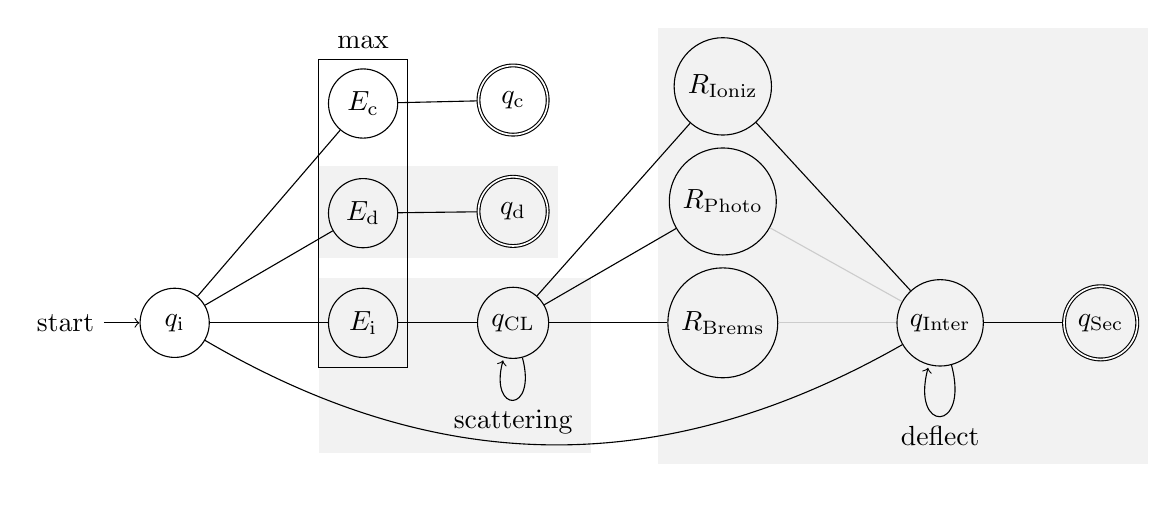
\begin{tikzpicture}

    \node[state ,initial]     (qi)              {$q_\mathrm{i}$};

    \node[state]   (Ei) [right= 1.5cm of qi] {$E_\mathrm{i}$};
    \node[state]   (Ed) [above= 0.5cm of Ei] {$E_\mathrm{d}$};
    \node[state]   (Ec) [above= 0.5cm of Ed] {$E_\mathrm{c}$};


    \node[state]   (qcl) [right= 1.0cm of Ei] {$q_\mathrm{CL}$};
    \node[state, accepting]   (qd) [above= 0.5 cm of qcl] {$q_\mathrm{d}$};
    \node[state, accepting]   (qc) [above= 0.5 cm of qd] {$q_\mathrm{c}$};

    \node[state]   (RBrems) [right= 1.5cm of qcl] {$R_\mathrm{Brems}$};
    \node[state]   (RPhoto) [above= 0.15cm of RBrems] {$R_\mathrm{Photo}$};
    \node[state]   (RIoniz) [above= 0.15cm of RPhoto] {$R_\mathrm{Ioniz}$};

    \node[state]   (qI) [right =1.5cm of RBrems] {$q_\mathrm{Inter}$};

    \node[state, accepting]   (qS) [right = 1.0cm of qI] {$q_\mathrm{Sec}$ };

    \path (qi) edge (Ei) edge (Ed) edge (Ec)

    (Ei)      edge                                    (qcl)
    (Ed)      edge                                    (qd)
    (Ec)      edge                                    (qc)

    (qcl)     edge                                    (RBrems)
    edge                                    (RPhoto)
    edge                                    (RIoniz)

    edge  [loop below] node (scatter) {scattering}    ()

    (RBrems)  edge  [color=black!20]                  (qI)
    (RPhoto)  edge  [color=black!20]                  (qI)
    (RIoniz)  edge                                    (qI)


    (qI)      edge                                    (qS)
    edge [loop below] node (deflect) {deflect}    ()
    (qI)      edge [bend left, below]                 (qi);


    \node [draw=black, rectangle, fit=(Ei) (Ed) (Ec), label=$\max$]{};

    \begin{scope}[on background layer]
        \node [fill=gray!10, rectangle, fit=(Ei) (qcl) (scatter)]{};
        \node [fill=gray!10, rectangle, fit=(Ed) (qd)]{};
        \node [fill=gray!10, rectangle, fit=(RBrems) (RIoniz) (RPhoto)
        (qI) (qS) (deflect)]{};
    \end{scope}

    % edge (RBrems)
    % edge (qI)
    % edge (qS);
\end{tikzpicture}
\end{document}
